  
\documentclass[a4paper, 11pt]{article}

\usepackage{graphicx}
\usepackage{subfigure}
\usepackage{amsmath}
\usepackage{color}
\usepackage{subscript}
% Use symbols like degrees
\usepackage{gensymb}
% In case we need to rotate a table
\usepackage{rotating}
% To insert code samples
\usepackage{listings}
\usepackage{tabularx}

% Change margins because article class is too small
\addtolength{\oddsidemargin}{-2cm}
\addtolength{\evensidemargin}{12cm}
\addtolength{\textwidth}{4cm}
\addtolength{\topmargin}{-3cm}
\addtolength{\textheight}{5cm}

% define some colors here if needed
\definecolor{_green}{rgb}{0,0.6,0}
\definecolor{_gray}{rgb}{0.5,0.5,0.5}
\definecolor{_mauve}{rgb}{0.58,0,0.82}
\definecolor{_lyellow}{rgb}{0.1,0.1,0.1}


\lstset{
  %rulecolor=\color{black},         % if not set, the frame-color may be changed on line-breaks within not-black text (e.g. comments (green here))
  tabsize=2,
  title=\lstname                    % show the filename of files included with \lstinputlisting; also try caption instead of title
  backgroundcolor=\color{white},  % choose the background color;
  language=C++,                     % the language of the code
  basicstyle=\ttfamily\small,       % the size of the fonts that are used for the code 
  aboveskip={1.0\baselineskip},
  belowskip={1.0\baselineskip},
  columns=fixed,
  extendedchars=true,               % lets you use non-ASCII characters; for 8-bits encodings only, does not work with UTF-8
  breaklines=true,                  % sets automatic line breaking
  tabsize=4,                        % sets default tabsize to X spaces
  prebreak=\raisebox{0ex}[0ex][0ex]{\ensuremath{\hookleftarrow}},
  frame=lines,                      % adds a frame around the code (eg. single)
  showtabs=false,                   % show tabs within strings adding particular underscores
  showspaces=false,                 % show spaces everywhere adding particular underscores; it overrides 'showstringspaces'
  showstringspaces=false,           % underline spaces within strings only
  keywordstyle=\color{_mauve},      % keyword style
  commentstyle=\color{_green},      % comment style
  stringstyle=\color{_gray},        % string literal style
  deletekeywords={...},             % if you want to delete keywords from the given language
  otherkeywords={*,...},            % if you want to add more keywords to the set
  numbers=left,                     % where to put the line-numbers;
  keepspaces=true,                  % keeps spaces in text, useful for keeping indentation of code (possibly needs columns=flexible)
  numberstyle=\footnotesize\color{_gray},% the style that is used for the line-numbers 
  stepnumber=1,                     % the step between two line-numbers.
  numbersep=5pt,                    % how far the line-numbers are from the code
  captionpos=t,                     % sets the caption-position bottom(b), top(t)
  escapeinside={\%*}{*)}            % if you want to add LaTeX within your code
}


\begin{document}
\title{Implementation of time-of-flight (TOF) in CASToR}
\maketitle

%---------------------------------------------------------------------------------------------------------------------------------------------------------------
\section{Index}

\noindent
\begin{tabularx}{\linewidth}{p{3cm}X}
TOF & time-of-flight \\
LOR & line-of-response \\
i & LOR or detector pair index \\
j & voxel index \\
$A_{ij}$ & element of the system matrix for voxel j and LOR i \\
$y_i$ & number of counts detected in LOR i \\
$N_j$ & number of voxels \\
$N_i$ & number of detector pairs or LORs \\
$\bar{r}_i$ & expected random counts rate for LOR i \\
$\bar{s}_i$ & expected scattered counts rate for LOR i \\
$\Delta t$ & TOF measurement (difference between arrival times of coincident photons)\\
$v$ & position on the LOR with respect to the LOR center\\
$c$ & speed of light\\
$b$ & TOF bin index, either cumulative bin (histogram data) or quantization bin (list-mode data with quantized TOF measurements)\\
$w$ & TOF weight multiplying the non TOF component of the system matrix ($A_{ij}$)
\end{tabularx}


%---------------------------------------------------------------------------------------------------------------------------------------------------------------
\section{Foreword}

This is a summary of implementation details for TOF reconstruction in CASToR. For more explanations about equations, see the technical note on TOF implementation by M. Filipovic et al., "Time-of-flight (TOF) implementation for PET reconstruction in practice", in print in "Physics in Medicine and Biology".

%---------------------------------------------------------------------------------------------------------------------------------------------------------------
\section{CASToR datafile}

In the TOF histogram data file
\begin{itemize}
\item (header) the TOF bin size (in ps) and the number of TOF bins must be provided
\item (binary) the estimation of the expected random counts rate should be provided per LOR ($\bar{r}_i$), as for non TOF data
\item (binary) the estimation of the expected scattered counts rate should be provided for each LOR and each TOF bin ($\bar{s}_{ib}$)
\end{itemize}

In the TOF list-mode data file
\begin{itemize}
\item (header) the range of TOF measurements (in ps) must be provided (usually equal to the coincidence timing window)
\item (header) the size of the TOF quantization bin (in ps) is optional, if provided the equation \ref{mlem_q_l} is used, otherwise the equation \ref{mlem_l} is used
\item (binary) the estimation of the expected random counts rate should be given per LOR ($\bar{r}_i$), as for non TOF data
\item (binary) the estimation of the expected scattered counts rate should be given for each LOR and each TOF measurement ($\bar{s}_{i}(v)$ or  $\bar{s}_{i}(v_b)$)
\end{itemize}

See also the data file documentation.

%---------------------------------------------------------------------------------------------------------------------------------------------------------------
\section{Definition}

The time-of-flight measurement $\Delta t$ is the difference of arrival times $t_1$ and $t_2$ of coincident photons into detection units $c_1$ and $c_2$, so positive $\Delta t$ is associated to annihilation events closer to $c_2$.

For reconstruction, $\Delta t$ is converted into $v$, the presumed spatial position of the annihilation on the LOR, given with respect to the center of the LOR, as

\begin{equation}
v = \frac{c\Delta t}{2}
\end{equation}

The spatial TOF uncertainty function is modeled as a Gaussian probability distribution with standard deviation $\sigma$, computed from the TOF resolution FWHM field given (in ps) in the input data file.

%---------------------------------------------------------------------------------------------------------------------------------------------------------------
\section{ML-EM equations}

%For TOF histogram data, the measured data are modelled with a Poisson distribution with expectation
%\begin{equation}
%\bar{y}_{ib}=\sum_{j}A_{ijb}\lambda_j+\bar{r}_{ib}+\bar{s}_{ib}
%\label{y_model}
%\end{equation}

For TOF histogram data
\begin{equation}
\lambda_j^{t+1}=\lambda_j^{t}\frac{1}{\sum_{ib} A_{ijb}}\sum_{ib}{A_{ijb}\frac{y_{ib}}{\sum_k{A_{ikb}\lambda_k^t+\bar{r}_{ib}+\bar{s}_{ib}}}}.
\label{mlem_h}
\end{equation}

\noindent For TOF list-mode data with quantized TOF measurements
\begin{equation}
\lambda_j^{t+1}=\lambda_j^{t}\frac{1}{\sum_{i=1}^{N_{LOR}} \int A^q_{ij}(v)\mathrm{d}v} \sum_{n=1}^{N_{coinc}}{A^q_{i_nj}(v_{b_n})\frac{1}{\sum_k{A^q_{i_nk}(v_{b_n})\lambda^t_k+\bar{r}^q_{i_n}(v_{b_n})+\bar{s}^q_{i_n}(v_{b_n})}}}
\label{mlem_q_l}
\end{equation}
equivalent to
\begin{equation}
\lambda_j^{t+1}=\lambda_j^{t}\frac{1}{\sum_{ib} A_{ijb}}\sum_{n=1}^{N_{coinc}}{A_{i_njb_n}\frac{1}{\sum_k{A_{i_nkb_n}\lambda_k^t+\bar{r}_{i_nb_n}+\bar{s}_{i_nb_n}}}}.
\label{mlem_q_h}
\end{equation}

\noindent For TOF list-mode data with continuous TOF measurements
\begin{equation}
\lambda_j^{t+1}=\lambda_j^{t}\frac{1}{\sum_{i=1}^{N_{LOR}} \int A_{ij}(v)\mathrm{d}v} \sum_{n=1}^{N_{coinc}}{A_{i_nj}(v_n)\frac{1}{\sum_k{A_{i_nk}(v_n)\lambda_k^t+\bar{r}_{i_n}(v_n)+\bar{s}_{i_n}(v_n)}}}.
\label{mlem_l}
\end{equation}

\subsection{System matrix}

TOF weights are a component of the system matrix for TOF reconstruction. They are independent of other components and thus multiply the non TOF part of the system matrix. Hence, the system matrix elements for TOF histogram data are $A_{ijb}=A_{ij}w_{ijb}$, for TOF list-mode data with continuous TOF measurements $A_{ij}(v)=A_{ij}w_{ij}(v)$, and for TOF list-mode data with quantized TOF measurements $A^q_{ij}(v_b)=A_{ij}w^q_{ij}(v_b)$.

There are several options for the computation of TOF weights, making trade-offs between speed and accuracy: truncation of the nominal Gaussian function, precomputation of the TOF weighting function vs computation on the fly, accurate vs approximate processing of TOF bins. They can be provided using -proj-common option (see also -help-projm for details).

For TOF list-mode data with continuous measurements, TOF weights are computed by simply sampling a Gaussian.
For TOF list-mode data with quantized measurements and for TOF histogram data, the TOF weights can be computed using one of the following formulas

\begin{align}
&\int \mathcal{N}(v|v_{j},\sigma)\Pi(v|v_b, \Delta v_b)\mathrm{d}v=h\int_{v_b-\Delta v_b/2}^{v_b+\Delta v_b/2} \mathcal{N}(v|v_{j},\sigma)\mathrm{d}v
\label{w_bin_int}\\
&=\Big(\mathcal{N}(\cdot|0,\sigma) \ast \Pi(\cdot|0, \Delta v_b)\Big)\Big(v_j-v_b\Big)
\label{w_bin_conv}\\
&\approx \mathcal{N}(v_b|v_{j},\sigma)h\Delta v_b \label{w_bin_approx}
\end{align}

where $\Pi$ is the TOF bin function defined as

\begin{equation}
\Pi_b(v)=
\begin{cases}
h &  \quad  v_b-\Delta v_b/2 < v \leq v_b+\Delta v_b/2 \\
0& \quad otherwise
\label{tof_bin}
\end{cases}
\end{equation}

with $h=1$ for TOF histogram data and $h=1/\Delta v_b$ for TOF list-mode data with quantized TOF measurements. See the PMB technical note for more details.

\begin{figure}[!htb]
\centering
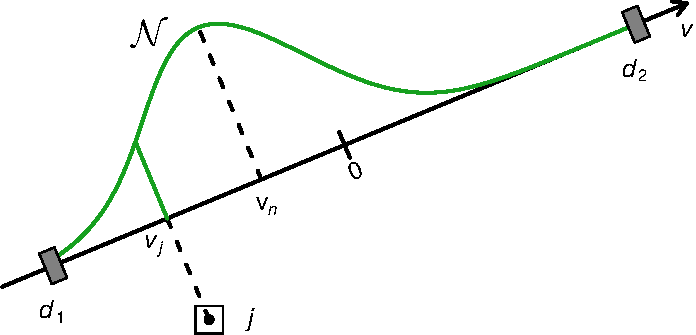
\includegraphics[width=0.3\textwidth]{figures/tof_weights_illustr1.pdf}
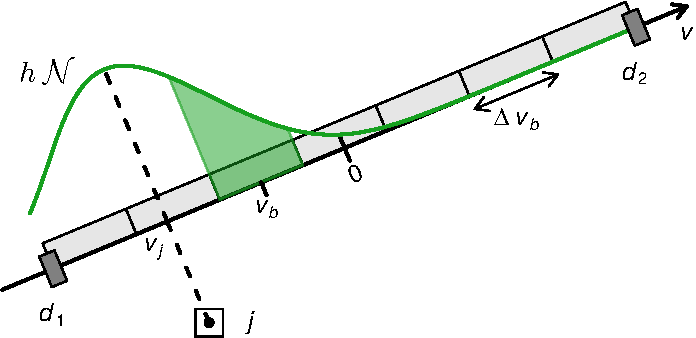
\includegraphics[width=0.34\textwidth]{figures/tof_weights_illustr2.pdf}
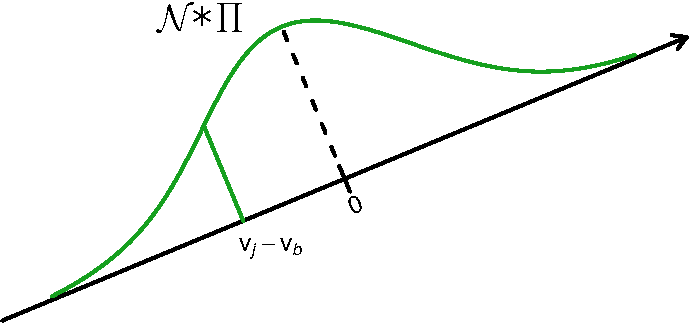
\includegraphics[width=0.3\textwidth]{figures/tof_weights_illustr3.pdf}
\caption{Illustration of the computation of TOF weights for continuous TOF measurements (left), for TOF bins using the equation \ref{w_bin_int} (center) and for TOF bins using the equation \ref{w_bin_conv} (right)}
\label{illustr_var}
\end{figure}

The equation \ref{w_bin_int} is used with options for accurate processing of TOF bins on the fly (without precomputation). The equation \ref{w_bin_conv} is used with options for accurate processing of TOF bins with precomputation. The equation \ref{w_bin_approx} is used with options for approximate processing of TOF bins, either with or without precomputation.

The precision of the precomputed TOF weighting function is currently hard coded at $1\mu m$.

%---------------------------------------------------------------------------------------------------------------------------------------------------------------
\section{Voxel sensitivity}

In theory, the voxel sensitivity is the same, regardless of the data format or the use of TOF.

\begin{equation}
\label{sens}
\sum_i A_{ij} = \sum_i\sum_b A_{ijb} = \sum_i \int{A_{ij}(v)\mathrm{d}v} = \sum_i \int{A^q_{ij}(v)\mathrm{d}v}.
\end{equation}

For TOF list-mode data, the voxel sensitivities are computed as for non TOF data, before the actual reconstruction and using the non TOF system matrix elements.

For TOF histogram data, the voxel sensitivities can be precomputed before the actual reconstruction using the non TOF system matrix elements, or they can be computed on the fly using the TOF system matrix elements (default behaviour, may not satisfy the equation \label{sens} if TOF weights are computed with approximations).

\section{Properties}

The following equations should be satisfied for the input TOF data.

\begin{equation}
\sum_b y_{ib} = y_i.
\label{y_sum}
\end{equation}

\begin{equation}
\sum_b \bar{r}_{ib} = \bar{r}_i \qquad , \qquad \int \bar{r}_i(v)\mathrm{d}v = \bar{r}_i
\end{equation}

\begin{equation}
\sum_b \bar{s}_{ib} = \bar{s}_i \qquad , \qquad \int \bar{s}_i(v)\mathrm{d}v = \bar{s}_i
\end{equation}

The following equations are satisfied within numerical limits when TOF weights are computed with the highest accuracy

\begin{equation}
\sum_b w_{ijb} = 1 \qquad\mbox{,}\qquad \int w_{ij}(v)\mathrm{d}v = 1 \qquad\mbox{,} \qquad \int w^q_{ij}(v)\mathrm{d}v = 1.
\label{w_sum}
\end{equation}


\subsection{Random and scatter counts}

For histogram TOF data, the estimation of the expected random counts rate is computed for each TOF bin by dividing the provided estimation per LOR $\bar{r}_i$ with the number of TOF bins. $\bar{r}_{ib}$ is thus the same for all TOF bins in a LOR. The estimation of the expected scattered counts rate is provided directly in the input data file for each LOR and each TOF bin.

For list-mode data, the estimation of the expected random counts rate is computed for each event by dividing the provided estimation per LOR $r_i$ with the spatial range of TOF measurements. The estimation of the expected scattered counts rate is provided directly in the input data file for each event.


\end{document}
